\begin{frame}{LoRa-Modulationstechnik: \alert{Chirp Spread Spectrum} (\alert{CSS})}
  \alert{Chirp Spread Spectrum} bzw.\ kurz \alert{CSS} ist eine Modulationstechnik, bei der \alert{sinusförmige} Signale verwendet werden, deren Frequenz sich im Zeitverlauf \alert{erhöht} \textbf{(\textcolor{fh-ooe-red}{Up-Chirp})} oder \alert{verringert} \textbf{(\textcolor{fh-ooe-red}{Down-Chirp})}.
  \begin{center}
    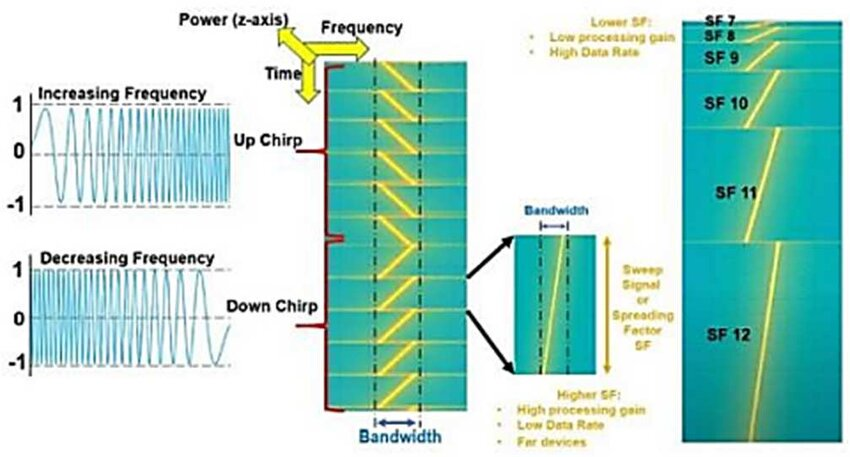
\includegraphics[width=0.7\textwidth]{material/LoRa-Chirp-Spread-Spectrum-Illustration-13.png}
  \end{center}
\end{frame}
